\RequirePackage{fix-cm}
%
%\documentclass{svjour3}                     % onecolumn (standard format)
%\documentclass[smallcondensed]{svjour3}     % onecolumn (ditto)
\documentclass[smallextended]{svjour3}       % onecolumn (second format)
%\documentclass[twocolumn]{svjour3}          % twocolumn
%
\smartqed  % flush right qed marks, e.g. at end of proof

\usepackage{graphicx}
\usepackage{mathptmx}      % use Times fonts if available on your TeX system
\usepackage{amsmath}
\usepackage{url}
\usepackage{bm}
\usepackage{amssymb}
\usepackage{natbib}

\newcommand{\beq}{\begin{equation}}
\newcommand{\eeq}{\end{equation}}
\newcommand{\pdif}[2]{\frac{\partial #1}{\partial #2}}
\newcommand{\pddif}[3]{\frac{\partial^2 #1}{\partial #2 \partial #3}}
\newcommand{\ts}{^T}

% Insert the name of "your journal" with
\journalname{Environ Ecol Stat}
%
\begin{document}

\title{Finite area smoothing with generalized distance splines}

%\titlerunning{Short form of title}        % if too long for running head

\author{David L. Miller         \and
        Simon N. Wood
}

%\authorrunning{Short form of author list} % if too long for running head

\institute{David L. Miller \at
              Department of Natural Resources Science, University of Rhode Island, Kingston, Rhode Island 02881, USA \\
              \email{dave@ninepointeightone.net}
           \and
           Simon N. Wood \at
              Department of Mathematical Sciences, University of Bath, Claverton Down, Bath BA2 7AY, UK
}

\date{Received: date / Accepted: date}
% The correct dates will be entered by the editor


\maketitle

\begin{abstract}
Most conventional spatial smoothers smooth with respect to the Euclidean distance between observations, even though this distance may not be a meaningful measure of spatial proximity, especially when boundary features are present. When domains have complicated boundaries leakage (the inappropriate linking of parts of the domain which are separated by physical barriers) can occur. To overcome this problem, we develop a method of smoothing with respect to generalized distances, such as within domain distances. We obtain the generalized distances between our points and then use multidimensional scaling to find a configuration of our observations in a Euclidean space of 2 or more dimensions, such that the Euclidian distances between points in that space closely approximate the generalized distances between the points. Smoothing is performed over this new point configuration, using a conventional smoother. To mitigate the problems associated with smoothing in high dimensions we use a generalization of thin plate spline smoothers proposed by \cite{Duchon:1977tr}. This general method for smoothing with respect to generalized distances improves on the performance of previous within-domain distance spatial smoothers, and often provides a more natural model than the soap film approach of \cite{Wood:2008vo}. The smoothers are of the linear basis with quadratic penalty type easily incorporated into a range of statistical models.
\keywords{Finite area smoothing \and generalized additive model \and multidimensional scaling \and spatial modelling \and splines.}
% \PACS{PACS code1 \and PACS code2 \and more}
% \subclass{MSC code1 \and MSC code2 \and more}
\end{abstract}

\section{Introduction \label{IN}}

In ecology one would often like to create a smooth map of some noisy response as a function of geographical coordinates. In such cases, care must be taken to account for the structure of the domain which is being modelled. If the domain is bounded (\textit{finite area smoothing}) then problems can occur when the smoother does not respect the boundary shape appropriately, especially when the shape of the boundary is complex. This complexity may manifest itself as some peninsula-like feature(s) in the domain with notably different observation values on either side of the feature. Features such as peninsulae give rise to a phenomenon known as \emph{leakage}. The top two panels of Figure \ref{leakage} show an example of leakage \citep[taken from][]{Wood:2008vo} where the high values in the upper half of the domain (top panel) leak across the gap to the lower values below and vice versa (second panel). The phenomenon is problematic since it causes the fitted surface to be mis-estimated; this can then lead to incorrect inference, in particular the mis-identification of ``hot spots'' in biological populations.

% leakage example 
\begin{figure}
\centering
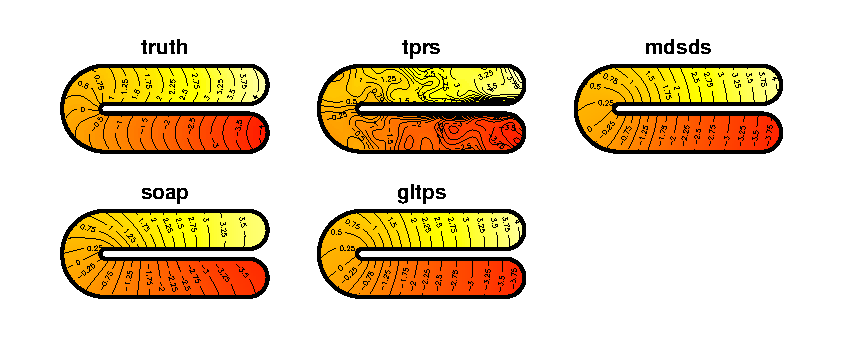
\includegraphics[width=\textwidth]{Fig1.eps}\\
\caption{Top row (left to right): the modified Ramsay horseshoe function from \protect\cite{Wood:2008vo}, predictions from models using thin plate regression splines (``tprs'') and MDSDS (``mdsds''). Bottom row: predictions from the soap film smoother (``soap'') and geodesic low-rank thin plate splines (``gltps''). Prediction were made from models where the data were 600 points were sampled from the horseshoe and standard normal noise was added. Note that the predicted surface from the thin plate regression spline fit shows severe leakage
\label{leakage}}
\end{figure}


The problem of leakage arises because spatial smoothers consider proximate data to be similar, but in almost all cases distance between data locations is measured using straight line (Euclidean) distance. This approach is flawed in cases in which Euclidean distance is not a meaningful measure of proximity. For example, since whales do not travel on land, the meaningful distance between sightings of two whales on either side of the Antarctic peninsula is not the straight line distance across the peninsula, but the shortest path between them that stays entirely in open water. This issue is ubiquitous in spatial ecology. Natural and man-made barriers carve up the landscape (and seascape), partitioning biological populations; spatial models should take this into account. 

In this article we propose a general method for smoothing, based on generalized distances between points. We apply this to produce a finite area smoother, based on the \textit{within-area distances} between points in the domain of interest. The general approach uses multidimensional scaling \citep[MDS; e.g.][Chapter 10]{chatfield1980introduction} to associate a location in a $\cal D$ dimensional Euclidian space ({\em p-space}) with each original data point. The Euclidian distances between points in p-space then approximate the original generalized distance between the points. Smoothing is then performed with respect to locations in p-space. Reasonable approximation of the generalized distances by the Euclidean distances in p-space can require $\cal D$ to be greater than the 2-4 dimensions in which conventional multidimensional smoothers work well. For this reason we revisit the general class of smoothers proposed in \cite{Duchon:1977tr}, selecting a smoother that behaves well with increasing dimension. Note that when applied to the finite area problem our generalized distance smoother can be viewed as an  extension of \cite{Wang:2007tf}, albeit somewhat better founded (which we argue below).

The use of multidimensional scaling in spatial statistics is not new, especially in the kriging literature. For example, \cite{Sampson:1992wm} model spatial covariance functions by computing a distance measure based on the observed spatial covariances, then project the points using MDS before kriging (points out of sample are found using a thin plate spline). Their approach differs from ours in a number of ways: (i) they require multiple observations at each location in order to calculate the covariances, (ii) only projections in 2 dimensions are considered and (iii) non-metric MDS is used. Further applications in geostatistics are described in Section \ref{conclusion} and compared to the method proposed here.

The smoother proposed here has the attractive property of being representable using a linear basis expansion with an associated quadratic penalty. Such basis-penalty smoothers have a dual interpretation as Gaussian random fields \citep{rue2005gaussian}, and are appealing because of the ease with which they can be incorporated as components of other models. For example, varying-coefficient models, random/mixed effects models and signal regression models, as well as the focus for this article: generalized additive models \citep[see e.g.][for overviews]{ruppert2003semiparametric, Wood:2006wz}. This flexibility is vital in ecological applications, where a spatial smooth is usually only one part of a much larger model.

Before presenting our proposed method in detail we now briefly review spline type spatial smoothers, and previous approaches to the finite area smoothing problem in the additive model literature.

\subsection{Spline smoothing for spatial data}

In the simplest case, we wish to find an $f$ which is a smooth function of spatial coordinates, $x_1$ and $x_2$. We model $f$ using a basis function expansion:
\begin{equation}
f(x_{1}, x_{2}) = \sum_{k=1}^K \beta_k b_k(x_{1}, x_{2}),
\label{basis-exp}
\end{equation}
where the $\beta_k$s are coefficients to be estimated and the $b_k$s are flexible (known) basis functions, such as thin plate spline basis functions or tensor products of B-splines. 

If $K$ is made large enough to avoid substantial model mis-specification bias, then the estimates of $f$ are almost certain to over-fit any data to which they are fitted. For this reason it is usual to associate a measure $J(f)$ of function wigginess with $f$, and to use this to penalize over fit during model estimation. 
For example, consider the simple generalized linear model  
$$
y_i \sim \text{EF}(\mu_i, \phi),~~~~ g(\mu_i) = \eta_i =f(x_{1i},x_{2i})
$$
where EF denotes an exponential family distribution with mean $\mu_i$ and scale parameter $\phi$, while $g$ is a known link function and $\eta_i$ is known as the `linear predictor' of $y_i$. Letting $l({\bm \beta})$ be the log likelihood then estimation of $\bm \beta$ is by maximization of 
$$
l({\bm \beta}) - \lambda/2 J(f)
$$ 
where $\lambda$ is a tune-able smoothing parameter, used to control the wiggliness of the estimate of $f$. $\lambda $ is typically estimated by GCV or marginal likelihood maximization \citep{Wood:ub}. A popular $J(f)$ in the spatial context is the 2 dimensional thin plate spline penalty
$$
J(f) = \int \left (\pdif{^2 f}{x_1^2}\right )^2 + 2\left ( \pddif{f}{x_1}{x_2}\right )^2 + \left (\pdif{^2 f}{x_2^2}\right )^2 dx_1 dx_2
$$
which can conveniently be written as a quadratic form in $\bm \beta$. 

Within this framework it is straightforward to allow $\eta_i$ to depend on multiple smooth functions of various predictor variables, as well as on conventional parametric terms that are linear in any unknown parameters \citep{hastie1990generalized}. Such models are widely used in quantitative ecology, for example in the creation of density maps which can then be integrated over the domain to obtain an abundance estimate \citep[e.g.]{Hedley:2004et, WILLIAMS:2011in} or as part of a larger model, taking into account nuisance spatial effects \citep[e.g.]{Augustin:2009ui}.

\section{Previous approaches to the problem of leakage}
\label{previous-approaches}

There 3 main types of existing approach to dealing with the finite area smoothing problem.

\subsection{Partial differential equation methods}

\cite{Ramsay:2002uo} exploited the link between smoothing with differential operator based penalties and partial differential equations to produce a smoother defined as the solution to a particular PDE problem defined only over a finite area. His FELSPINE method uses a finite element method to compute a smoother, based on the penalty 
\beq
J(f) = \int_\Omega \left ( \pdif{^2 f}{x_1^2} + \pdif{^2 f}{x_2^2} \right )^2 dx_1 dx_2 
\label{soap}
\eeq 
Where $\Omega$ is the region of the $x_1$, $x_2$ plane of interest. Ramsay had to use the very strong boundary condition that contours of $f$ meet the boundary of $\Omega$ at right angles, which leads to artefacts when the condition does no hold (see Wood et al, 2008). The computational method also makes it awkward to include such terms in larger models.

\cite{Wood:2008vo} use the physical analogy of a soap film to motivate an alternative which can be represented as a basis penalty smoother, and has better boundary behaviour. First consider the domain boundary to be made of wire, then dip this wire into a bucket of soapy water; a soap film with the same shape as the boundary will have then formed. If the wire lies in the spatial plane, the height of the soap film at a given point is the value of the smooth at that point. This film is then distorted smoothly toward each datum, while minimising the overall surface tension in the film. Mathematically the soap film consists of two sets of basis functions, one that is based entirely inside the domain (a set of interior knot locations are specified) and one that is induced by the (known or estimated) boundary values. These functions are found by solving Poisson and Laplace's equations in two dimensions. The penalty associated with the former set is again (\ref{soap}). 

The soap film approach has the basis-penalty form that is convenient for applied work and solves the boundary leakage problem, but basis setup is quite computationally expensive, and for many applications the approach is less natural than smoothing using within domain distances. A further problem with the soap film approach is that no distinction exists between `open' boundaries (for example a boundary that is simply the limit of the region surveyed) and `hard' boundaries (real physical barriers).

\subsection{Within-area distances}

\cite{Wang:2007tf} propose to replace straight-line distances with `geodesic' distances in a smoother that is a sort of approximate thin plate spline (Geodesic Low-rank Thin Plate Splines, GLTPS). To calculate the geodesic distances, a graph is constructed in which each vertex is the location of an observation and is connected only to its $k$ nearest neighbours. The within-area distances between each vertex pair is approximated using  Floyd's algorithm \citep{Floyd:1962:A9S:367766.368168} to find the shortest path through the graph. This algorithm is cubic in the number of data, making the approach costly for large datasets. At large sample sizes the geodesic distances will tend towards `within-area distance', i.e. the shortest path between two points that lies entirely within the domain of interest \citep{Bernstein:2000tp}.

Wang and Ranalli use their geodesic distances in place of the usual Euclidean distances in the radial basis functions used to define a thin plate spline. They leave the basis for the null space of the thin plate spline penalty unchanged, so some linkage across boundary features remains in the smoother. The principle difficulty in interpreting the results of their method is that it is unclear what their penalty term penalizes. The interpretational difficulty arises because  Wang and Ranalli's expressions (3) and (9) involve the square roots of matrices that are not positive semi-definite. In the case of their expression (3), which relates to a thin plate spline, this problem would be rectifiable if the spline coefficients had the usual thin plate spline linear constraints applied in order to force positive definiteness on the spline penalty. However in the case of (9), which defines their geodesic splines, there appears to be no sensible way to obtain positive semi-definiteness. This is a problem because matrix square roots in general only exist for positive semi-definite matrices plus some rather special cases not useful here \citep[see e.g.]{Higham1987405}. It appears that for computational purposes Wang and Ranalli have used the generalization of a matrix square root given in appendix A.2.11 of \cite{ruppert2003semiparametric}, but this square root lacks the basic properties that would allow Wang and Ranalli's (2) to be interpretable exactly as a (reparameterized) thin plate spline, or for it to be possible to work out what the penalty on their geodesic spline is actually penalizing. 

\cite{ScottHayward:2011tc} propose the Complex Region Spatial Smoother (CReSS) adapting GLTPS in two ways. First, in building the graph, edges are only drawn between two points if the straight line drawn between the points lies entirely within the boundary (boundary vertices are also included, in addition to observations). Second, a set of local radial basis functions are used (with a tuneable parameter controlling the locality of the basis). An AICc-weighted average over a series models with different basis sizes, knot locations and locality of the basis functions is used for prediction. Unlike Wang and Ranalli, the nullspace of the basis is removed.

The combination of an un-modified null space, the opacity of the penalty meaning and $O(n^3)$ computational cost of distance calculation are of some concern for practical work. In the case of CReSS, the necessity of running many models also creates a substantial computational burden. For both interpretive and computational reasons it seems worthwhile to investigate alternative ways of using the within-area distance idea, avoiding these difficulties.

\subsection{Domain warping}

Paul Eilers (in a seminar at University of Munich in 2006) suggested conformally mapping the smoothing domain to a convex one  via the Schwarz-Christoffel transformation \citep{Driscoll:2002tq}. The idea is that smoothing can then be conducted on the convex domain, without leakage problems. The first author has extensively investigated such an approach \citep[Chapter 3]{Miller:2012wy}, but there are insurmountable difficulties associated with the extreme modification of inter-observation distances necessary to achieve domain convexity, which cause artefacts that are significantly more problematic than the leakage effects that the method seeks to avoid. 

The methods proposed in the next section can be viewed as an attempt to put within-area distance methods on a more interpretable foundation by using an extension of the notion of domain warping. 


\section{The generalized distance smoothing model}
\label{proposed-model}

We assume that we want to model a response $y_i$ which is dependent on covariates via a linear predictor $\eta_i$. Our model is then
$$
\eta_i = \alpha_i + f({\bf d}_i)
$$
where $\alpha_i$ may depend linearly on further model coefficients (or may simply be zero). $f$ is a smooth function, dependent on ${\bf d}_i$, a vector of generalized distances between the $i^{\rm th}$ observation and either i) the other observations, or ii) some set of `reference points'. 

We complete the model by setting 
$$
f({\bf d}_i) = f_{\cal D}\{{\bf x}({\bf d}_i)\}
$$
where ${\bf x}({\bf d})$ is the location of the point with distance vector $\bf d$ in the $\cal D$ dimensional 
Euclidean space determined by multi-dimensional scaling applied to either i) the matrix for the complete data set or ii) the distance matrix for the set `reference points' (see below). $f_{\cal D}$ is a $\cal D$ dimensional \textit{Duchon spline} \citep{Duchon:1977tr}, a generalization of the familiar thin plate spline. 

The key idea here is that we smooth over a Euclidean space  in which the Euclidean inter-observation distances are approximately equal to the original generalized distances. That is  $\|{\bf x}({\bf d}_i) - {\bf x}({\bf d}_j) \| \approx d_{ij}$ when $d_{ij}$ is the generalized distance between points $i$ and $j$ ($\|\cdot \|$ is the Euclidean norm). The choice of $\cal D$ determines the accuracy of the distance approximation. This can either be part of model specification, in which case $\cal D$ is chosen to achieve some specified level of approximation accuracy, or more pragmatically, can be chosen to optimize estimated prediction error (e.g. GCV score).

In the case of finite area smoothing, the elements of ${\bf d}_i$ are `within-area' distances between points, that is to say the shortest path between two points, such that the path lies entirely within the domain of interest. We will refer to the original 2 dimensional data co-ordinates as being elements of the `o-space' while $\cal D$ dimensional co-ordinates in the MDS projection will be referred to as elements of the `p-space'. Web Appendix B gives and algorithm for calculating within-area distances for simple polygons. 

These smoothers will be henceforth referred to as MDSDS (Multi-Dimensionally Scaled Duchon Splines), and the next three subsections provide the details for the MDS, smoothing and $\cal D$ selection steps.

\subsection{MDS as a transformation of space}

In this section we consider the construction of the mapping ${\bf x}({\bf d})$ by multidimensional scaling \citep[MDS;][]{Gower:1968to}. We start the process by choosing a representative set of locations of size $n_s$ within the domain of interest (i.e. in o-space). This set might be all the locations at which we have observations, but in the case of finite area smoothing we would usually choose a set of locations spread uniformly over the region of interest in order to ensure that all the important geographic features in o-space will be represented in p-space. 

The generalized distances between all pairs of points in the representative set are then computed, in order to obtain a matrix $\bf D$ such that $D_{ij}$ is the squared generalized distance between points $i$ and $j$. MDS then finds a configuration of points in $\cal D$ dimensional Euclidean space such that the Euclidean distances between the points approximate the original generalized distances. The recipe for achieving this is straightforward. Defining ${\bf H} = {\bf I} - {\bf 11}\ts/n_s$ (where {\bf 1} is a vector of $1$s) we can obtain the double centred version of ${\bf D}$, ${\bf S} = - {\bf HDH}/2$, which is then eigen-decomposed
$$
{\bf S} = {\bf U}{\bm \Lambda}{\bf U}\ts.
$$ 
The rows of  ${\bf X }= {\bf U}{\bm \Lambda}^{1/2}$ then give locations in Euclidean space, such that the interpoint Euclidean distances in that space approximate the original generalized distances. The dimension of the resulting space is at most $n_s$ however, in practice not all of the eigenvalues of ${\bf S}$ may be positive. Using the first $\cal D$ columns of $\bf X$ gives a $\cal D$ dimensional p-space. See e.g. \cite[Chapter 10]{chatfield1980introduction} for more details.

We then require some means for finding the location in p-space of a point in o-space that was not used to calculate $\bf D$. Let $\bf d$ be the $n_s$ vector of squared generalized distances (in o-space) between this new point and the points in the original representative set. \cite{Gower:1968to} gives the following interpolation formula for the location of the new point in p-space 
$$
{\bf x} = - {\bm \Lambda}^{-1/2} {\bf U}\ts {\bf d}^\prime
$$
where $d^\prime_i = d_i - S_{ii}$. Again, $\bf x$ would usually be truncated, retaining only its first $\cal D $ components. 

So, MDS combined with Gower's interpolation formula provide a means for constructing and computing with ${\bf x}({\bf d})$. We now turn to the construction of a suitable smoother in p-space.

\subsection{Smoothing with Duchon splines}
\label{ss:duchon}

In order for our smoother to have a convenient basis-penalty form, we need to smooth in p-space using a basis-penalty smoother. A thin plate spline (TPS) is the obvious choice for smoothing arbitrarily scattered data where the Euclidean distance between points determines similarity, but there is a technical problem. To achieve a smooth $f$ requires $2m > {\cal D}$ where $m$ is the order of differentiation in the TPS penalty and the dimension of the space of unpenalized functions in a TPS basis is $M = \left ( \begin{array}{c} m + {\cal D} - 1 \\ {\cal D} \end{array} \right )$. As Figure \ref{nullspace-dim} shows the minimum possible $M$ increases rapidly with $\cal D$, leading to the danger of substantial undersmoothing as $\cal D$ increases.

\begin{figure}
\centering
\includegraphics[width=3in]{Fig2.eps} \\
\caption{Relationship between smoothing dimension ($d$) and the nullspace dimension ($M$) when $m$ (the derivative penalty order) is set to 2 for thin plate regression splines (dashed) and Duchon splines (solid). Note that as the nullspace dimension increases, the complexity of those functions in the nullspace increases too. For the thin plate splines a combination of the continuity condition that $2m>d$ and the form of $M$ makes the size of the nullspace increase very quickly with smoothing dimension}
\label{nullspace-dim}
% generated by thesis/mds/figs/nullspace-dim.R
\end{figure}

To combat this problem we use a more general version of the thin plate spline from the larger class of functions considered in \cite{Duchon:1977tr}, which will allow us to obtain a smoother for which $M = {\cal D} + 1$. This larger class has been almost entirely ignored in the statistical literature, so we provide a brief summary here. 

The difference between general Duchon splines and thin plate splines is in the smoothing penalty used. To understand the difference it helps to start with the general TPS penalty
\begin{equation}
J_{m,{\cal D}} = \int_{\mathbb{R}^d} \sum_{\nu_1 + \dots + \nu_d=m} \frac{m!}{\nu_1! \dots \nu_d!} \left( \frac{\partial^m f \left (\mathbf{x} \right )}{\partial x_1^{\nu_1} \ldots  \partial x_d^{\nu_d}} \right)^2 \text{d} x_1 \ldots  \text{d} x_d.
\label{tprs-pen}
\end{equation}
By Plancherel's theorem \citep[e.g.][p. 180]{vretblad2003fourier}, if we take the Fourier transform, $\mathfrak{F}$, of the derivatives in (\ref{tprs-pen}) then the penalty can be re-expressed as
\begin{equation}
J_{m,{\cal D}} =  \int_{\mathbb{R}^d} \sum_{\nu_1 + \dots + \nu_d=m} \frac{m!}{\nu_1! \dots \nu_d!} \left ( \mathfrak{F} \frac{\partial^m f}{\partial x_1^{\nu_1} \ldots  \partial x_d^{\nu_d}} \left (  \boldsymbol{\tau}\right ) \right )^2 \text{d} \boldsymbol{\tau},
\label{tprs-pen-ft}
\end{equation}
where $\bm \tau$ are now frequencies, rather than locations. Duchon then considers weighting the Fourier transform of the derivatives by some power of frequency, effectively increasing the penalization of high frequency components in the spatial derivatives if the power is positive. The resulting penalty is 
\begin{equation}
\breve{J}_{m,{\cal D}} = \int_{\mathbb{R}^d} \| \boldsymbol{\tau} \|^{2s} \sum_{\nu_1 + \dots + \nu_d=m} \frac{m!}{\nu_1! \dots \nu_d!}\left ( \mathfrak{F} \frac{\partial^m f}{\partial x_1^{\nu_1} \ldots  \partial x_d^{\nu_d}} \left (\boldsymbol{\tau} \right ) \right )^2 \text{d} \boldsymbol{\tau}.
\label{duchon-penalty}
\end{equation}
where $-{\cal D} < 2s < {\cal D}$ and the restriction $m + s > {\cal D}/2$ is applied to ensure continuity of the splines that result from use of this penalty. 

Duchon shows that the function minimising (\ref{duchon-penalty}) while interpolating or smoothing data at locations ${\bf x}_i$ has the form 
$$
f({\bf x}) = \sum_i^n \gamma_i K_{2m+2s-{\cal D}}(\|{\bf x}-{\bf x}_i\|) + \sum_j^M \alpha_j \phi_j({\bf x})
$$
where the $\phi_j({\bf x})$ form a basis for the polynomials of order $<m$, ${\bf x}_i$ is the $i^\text{th}$ observation location and $\gamma_i$ and $\alpha_j$ are coefficients to be estimated, subject to the $M$ linear constraints
\beq
\sum_i^n \gamma_i \phi_j({\bf x}_i)=0.
\label{duchon.constraint}
\eeq
The other basis functions are given by
$$
K_d(t) = \left \{ \begin{array}{ll}
(-1)^{(d+1)/2}|t|^d & d \text{~~odd}\\
(-1)^{d/2}|t|^d\log |t| & d \text{~~even}
\end{array} \right .
$$
Finally, given the linear constraints (\ref{duchon.constraint}),
$$
\breve{J}_{m,{\cal D}} = {\bf \delta} \ts {\bf K} {\bf \delta}
$$
where $K_{ij} = K_{2m+2s-{\cal D}}(\|{\bf x}_i-{\bf x}_j\|)$. Notice that $s=0$ gives a conventional TPS.

As an example of using this basis and penalty, we note that estimating $f$ to minimize
$$
\sum_i^n (y_i - f({\bf x}_i))^2 + \lambda \breve{J}_{m,{\cal D}}
$$
now reduces to the straightforward optimization problem of finding $\hat {\bm \gamma} $ and $\hat {\bm \alpha}$ to minimize
$$
\|{\bf y} - {\bf K } {\bm \gamma} - {\bf A}{\bm \alpha}  \|^2 + \lambda {\bm \gamma}\ts {\bf K} {\bm \gamma} ~~\text{s.t.}~~{\bf A}\ts {\bm \gamma} = {\bf 0}
$$
where $A_{ij} = \phi_j({\bf x}_i)$. Notice that this problem has exactly the same structure as the TPS problem, so exactly the same approach to computation can be taken. More importantly optimal rank reduced versions of these Duchon splines can be produced using the methods given in \cite{Wood:2003tc} for the TPS. \cite{Wood:2003tc} uses an eigen approximation to the full spline thereby avoiding the difficult problem of $\cal D$ dimensional knot placement that complicates other approaches to reduced rank splines, so we use this approach in what follows.

We are now in a position to produce a spline suitable for smoothing in p-space. Specifically we choose a (reduced rank) Duchon spline with $m=2$ and $s = {\cal D}/2 - 1$, which will give us a smooth $f$ for which $M={\cal D}+1$ (i.e. the unpenalized component of $f$ grows only linearly with $\cal D$).

\subsection{Selecting $\cal D$}
\label{s:mdsdimselect}

An obvious question is whether we actually need $\cal D$ to be larger than 2 in practice. Figure \ref{wt2-plot} provides an illustration that in general we do. It shows what happens when within-area distances over a 2 dimensional domain with a peninsulae are used to obtain a 2D p-space. Some of the points in the resulting p-space configuration become quite severely squashed together. In fact truncating the projection to two dimensions can sometimes cause the basic ordering of the points to be lost, making the task of the smoother impossible. Further investigation showed that increasing the dimensionality of p-space maintains the ordering of the points, however the number of dimensions required varied according to the shape of the domain. Increasing the dimension of p-space also makes the distances measured in p-space approximate the distance matrix, $\mathbf{D}$, better.

\begin{figure}
\centering
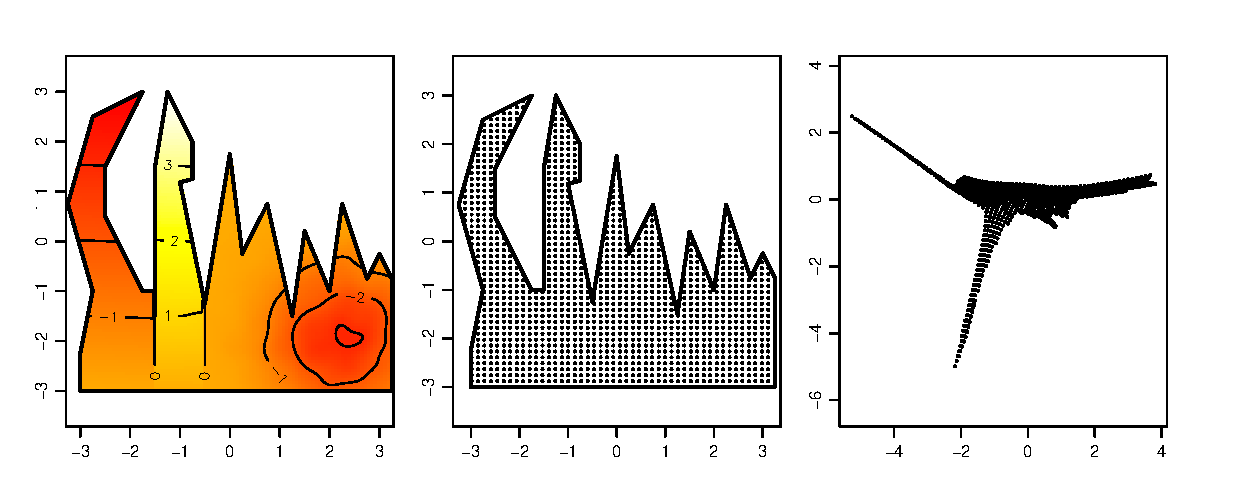
\includegraphics[width=\textwidth]{Fig3.eps} \\
\caption{Left to right: Test function over the peninsulae domain, points in the domain and finally their projection into 2-dimensional p-space when within-area distances are used to calculate the distance matrix. The p-space plot shows that some squashing can happen in two dimensions. The large left peninsula and some of the smaller peninsulae have lost their `width' and, in fact, points within them have lost ordering}
\label{wt2-plot}
% generated by examples/wt2/wt2-plot.R
\end{figure}

Having accepted the need for ${\cal D}>2$, we need some means of choosing $\cal D$. Rather than setting a maximum difference between the distances in $\mathbf{D}$ and the distances in the projection, we choose $\cal D$ in order to minimize GCV. Selecting $\cal D$ is typically a small part of the computational burden, since the MDS and smoothing are cheap relative to the computation of distances (at least in the finite area smoothing case). Figure \ref{aral-gcvplot} shows the relationship between $\cal D$ and GCV score for the Aral sea data analysed below. 


\section{Examples}
\label{examples}

To illustrate the utility of the model two simulation studies are shown, followed by examples using real data. All concentrate on the finite area smoothing problem. In each case MDSDS was compared with thin plate splines as described in \cite{Wood:2003tc} (which do not account for the boundary), geodedic low-rank thin plate splines (GLTPS) and the soap film smoother (which both do account for the boundary). The GLTPS model was as described in \cite{Wang:2007tf}, but with the within-area distances calculated as described in Web Appendix B (i.e. the same as for MDSDS); knots were placed using the \texttt{cover.design} method in the package \texttt{fields} \citep[again, as in][]{Wang:2007tf}. In all cases smoothing parameters were selected by GCV. The \textsf{R} packages \texttt{mgcv} (available from CRAN) and \texttt{msg} (available from \url{https://github.com/dill/msg}) were used to fit the models. Code for fitting the GLTPS is available at \url{https://github.com/dill/gltps}

In all the cases below the basis size specified refers to the maximum basis size allowed, since the penalty will reduce the complexity of the smoother, we simply need to specify an upper bound on the basis size.


\subsection{Ramsay's horseshoe}

The horseshoe shape shown in the top panel of Figure \ref{leakage} is an obvious benchmark for techniques that wish to combat leakage. Although perhaps unrealistic (and bordering on pathological), any new method that works well on the horseshoe should have a good chance of working well in more realistic situations. A simulation experiment was run with the same setup as in \cite{Wood:2008vo}: 200 replicates were generated at each of three error levels (standard normal noise multiplied by 0.1, 1 and 10) with sample size 600. A thin plate regression spline, with basis size 100 and a soap film smoother with 32 interior knots  and a 40 knot cyclic  spline was used to estimate the boundary. For the MDSDS model, the basis size was set to 100 and a 20 by 20 initial grid was used for the MDS projection (see Web Appendix A), MDS projection dimension was selected by GCV in the range of 2 and the number of dimensions that explained 95\% of the variation in the distance matrix of the initial grid. For the GLTPS 40 knot locations were selected as in \cite{Wang:2007tf}. For each realisation the mean squared error (MSE) was calculated between the true function and a prediction grid of 720 points.

\begin{figure}
\centering
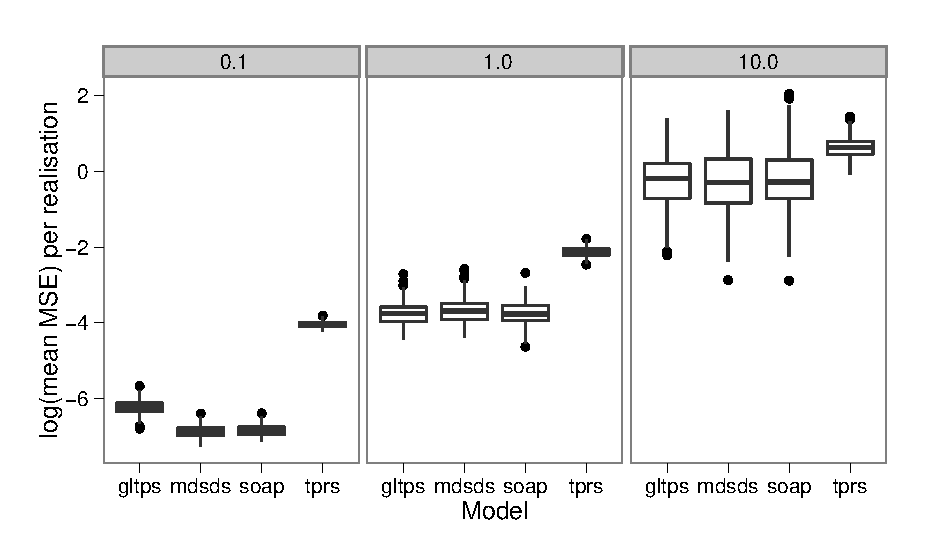
\includegraphics[width=\textwidth]{Fig4.eps}
\caption{Top: boxplots of per-realisation log mean squared error at the three noise levels. Using a paired Wilcoxon signed-ranks test, the difference between the new approach (``mdsds'') and the other models was significantly different for the two lower noise levels (at the 0.05 level). For the higher noise level, the three methods that accounted for the boundary (``gltps'' and ``soap'') were not distinguishable from MDSDS. The thin plate regression spline (``tprs'') was worse
\label{ramsay-results}}
% generated by examples/ramsay/ramsay-plot.R
\end{figure}

As can be seen in Figure \ref{ramsay-results}, the thin plate regression spline has rather poor performance in MSE terms while MDSDS, the soap film smoother and GLTPS perform significantly better. MDSDS performs better than the soap film smoother and GLTPS at lower noise levels, becoming indistinguishable at the highest noise level. The median number of dimensions selected for the MDS projection using GCV was 3 (max. 14, min. 2). Looking more qualitatively at the bottom three plots in Figure \ref{ramsay-results}, the predictions do not show any evidence of leakage.

% Wilcoxon vs. MDSDS
%tprs noise= 0.1 -1 p= 1.447002e-34 
%soap noise= 0.1 -1 p= 7.672467e-07 
%gltps noise= 0.1 -1 p= 1.447002e-34 
%tprs noise= 1 -1 p= 1.447002e-34 
%soap noise= 1 1 p= 0.003321106 
%gltps noise= 1 1 p= 0.0003642348 
%tprs noise= 10 -1 p= 5.060672e-25 
%soap noise= 10 -1 p= 0.8533422 
%gltps noise= 10 -1 p= 0.05883376 

\subsection{Peninsulae domain}

The results from the modified Ramsay horseshoe are encouraging. However the domain is not particularly realistic. To further explore the performance of MDSDS a more realistic domain was used. The domain, which attempts to mimic a coastline, is shown in the left panel of Figure \ref{wt2-plot}.

Simulations were run at signal-to-noise ratios of 0.50, 0.75 and 0.95 (equating to adding standard normal noise multiplied by 0.35, 0.9 and 1.55, respectively). The soap film smoother used 109 internal knots and 60 for the cyclic boundary smooth. The MDSDS models used an initial grid of 120 by 126 points, the basis size was 140. The thin plate regression spline basis size was also 140. For the GLTPS, 80 knots were selected using the space filling design.

Figure \ref{wt2-boxplots} shows the boxplots of the $\log$ of the MSE per realisation for each model. In the low noise cases, a paired Wilcoxon signed-ranks test showed that the soap film smoother and MDSDS were not significantly different at the 0.05 level. In all cases MDSDS was significantly better than both GLTPS and thin plate regression splines.

% Wilcoxon vs. MDSDS
%tprs noise= 0.35 -1 p= 7.969241e-31 
%gltps noise= 0.35 -1 p= 1.298381e-14 
%soap noise= 0.35 -1 p= 0.1789427 
%tprs noise= 0.9 -1 p= 1.903392e-28 
%gltps noise= 0.9 -1 p= 1.032922e-11 
%soap noise= 0.9 -1 p= 1.23365e-11 
%tprs noise= 1.55 -1 p= 9.46488e-32 
%gltps noise= 1.55 -1 p= 0.01354858 
%soap noise= 1.55 -1 p= 0.01313839 

\begin{figure}
\centering
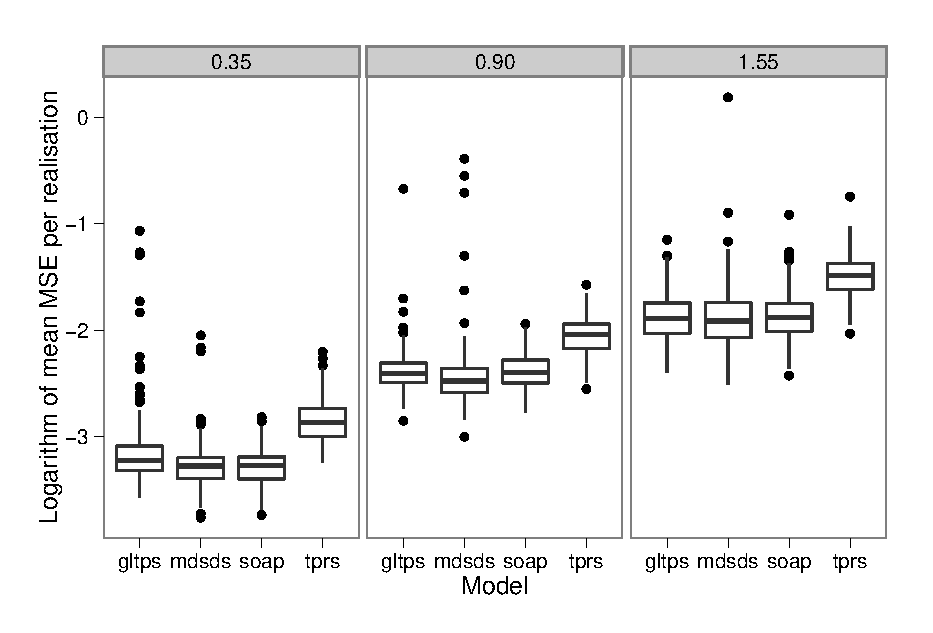
\includegraphics[width=\textwidth]{Fig5.eps} \\
\caption{Boxplots of logarithm of mean MSE per realisation for the models tested on the peninsulae domain at three noise levels. At each noise level, the median mean MSE was lower for MDSDS than for the thin plate regression spline, soap film smoother and GLTPS. A paired Wilcoxon signed-ranks test showed that the only significant difference (at the 5\% level) occurred between MDSDS and the soap film smoother at the 0.35 noise level}
\label{wt2-boxplots}
% generated by examples/wt2/wt2-boxplot.R
\end{figure}


\subsection{Aral sea}

The Aral sea is located between Kazakhstan and Uzbekistan and has been steadily shrinking since the 1960s when the Soviet government diverted the sea's two tributaries in order to irrigate the surrounding desert. The NASA SeaWifs satellite collected data on chlorophyll levels in the Aral sea over a series of 8 day observation periods from 1998 to 2002 \citep{Wood:2008vo}. The 496 data are averages of the $38^\text{th}$ observation period. Smooths were fitted to the spatial coordinates (Northings and Eastings; kilometres from a specified latitude and longitude) with the logarithm of chlorophyll concentration (modelled with a Gamma distribution) as the response.

The models that were fitted to the data were: a thin plate regression spline with basis size 70, MDSDS with a basis size of 70 (a 20 by 20 initial grid was used for the MDS projection), a GLTPS with 60 knots and soap film using 49 boundary knots and 74 internal knots. Using GCV for MDS projection dimension selection lead to a 5-dimensional projection. A plot of the relationship between projection dimension and GCV score can be seen in Figure \ref{aral-gcvplot}; there is a clear minimum at 5 dimensions.

\begin{figure}
\centering
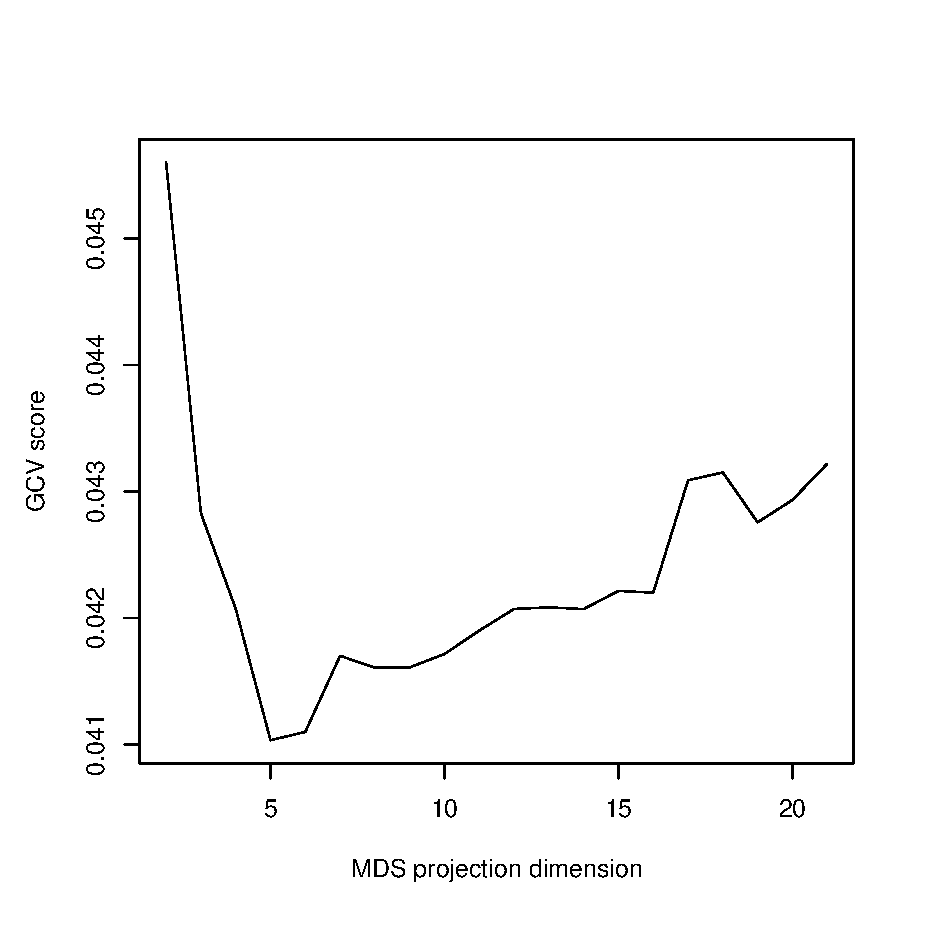
\includegraphics[width=3.5in]{Fig6.eps} \\
\caption{Plot of the relationship between GCV score and MDS projection dimension for the Aral sea data set. Here a clear minima at 5 dimensions can be seen, however there is no particular reason to believe that there will always be such a pronounced optima}
\label{aral-gcvplot}
% generated by examples/aral/aral-plot.R
\end{figure}

Predictions from the models over a grid of 496 points are shown in Figure \ref{aral-plot}. The fits are broadly similar across most of the domain. MDSDS, GLTPS and the soap film smoother do not show signs of leakage around (-50,-50), as the thin plate regression spline does.

\begin{figure}
\centering
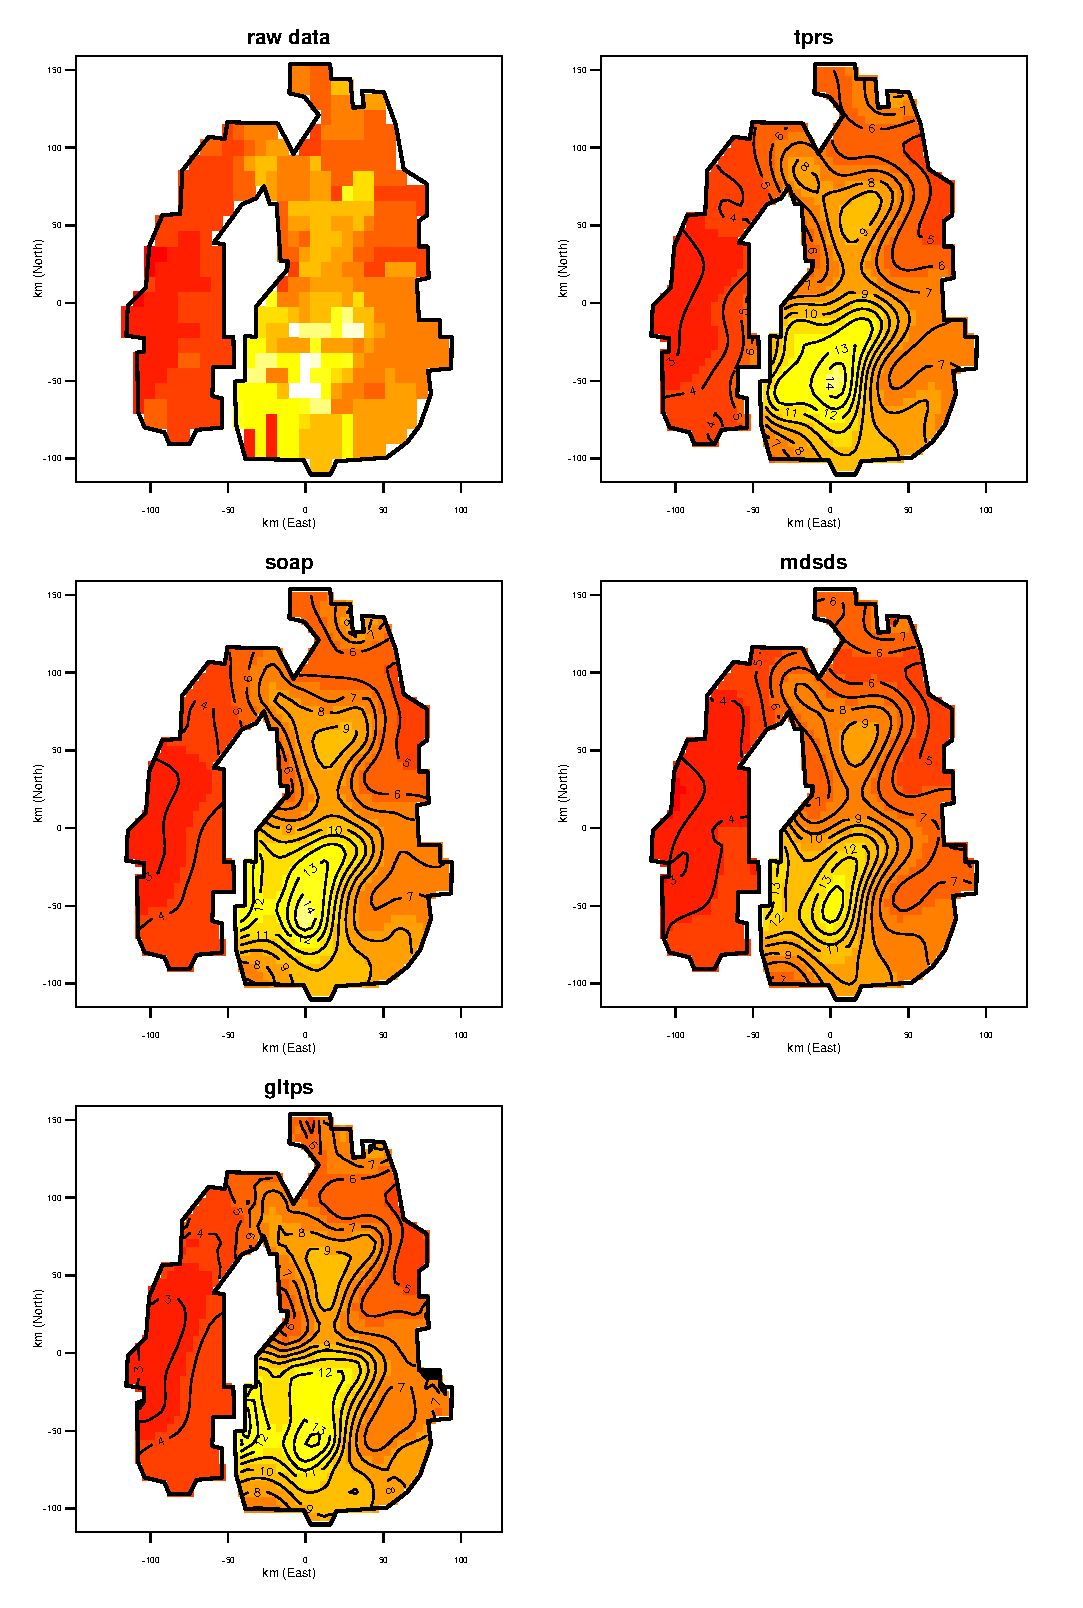
\includegraphics[height=0.8\textheight]{Fig7.eps}
\caption{Predictions from models of the Aral sea chlorophyll data. Top row, left to right: raw data, predicted surface for thin plate regression spline. Second row: predicted surfaces for the soap film smoother and MDSDS. Bottom row: predicted surface for GLTPS. The latter three avoid the leakage seen in the $(-50, 50)$ region of the thin plate regression spline fit}
\label{aral-plot}
% generated by examples/aral/aral-plot.R
\end{figure}

\section{Discussion}
\label{conclusion}

Our MDSDS approach appears to have competitive performance compared to existing methods, while providing a number of possible advantages. Relative to the soap film smoother the method has a more natural handling of open and closed boundaries, and is also often the more natural model when the linkage between geographic areas is via movement of organisms. Relative to \cite{Wang:2007tf} our approach is somewhat more transparent in terms of what is being penalized when smoothing, and also uses a null space basis that avoids leakage, unlike the Wang and Ranalli method for which the null space does not respect boundary features. As mentioned above, MDSDS fits easily into a generalized additive model, which may have many more components, which are often necessary for ecological work.

As mentioned above, using MDS to build covariance functions for kriging as been investigated previously. When non-Euclidean distances are used, covariance functions may no-longer be positive definite or conditionally negative definite \citep{Curriero:2005ww}, so MDS can be used to project the data, creating a set of Euclidean distances. For example, \cite{Loland:2003tp} used river network distances in the construction of a variogram, and overcame the problem of lack of positive definiteness by using MDS and then constructing the variogram in MDS space. Projection dimension selection is partially addressed in \cite{Jensen:2006kn}, the authors suggest using the proportion of variation explained or the Bayesian criterion of \cite{Oh:2011ve} as possible metrics but do not fully explore the issue, resorting to 2-dimensional projections. The use of Duchon splines in MDSDS allows for a high-dimensional projections, thus allowing for more accurate approximation of the distance matrix whilst ensuring that the points maintain ordering (this second point has not been addressed in the kriging literature to our knowledge).

Further work would involve considering more biologically motivated measures of distance. For example, distances based on the minimum energetic cost of moving between  two locations. It is also of interest to investigate the use of MDSDS for smoothing non-geographic distances outside of ecology such as the socio-economic similarity of parliamentary constituencies, or measures of genetic relatedness.

\begin{acknowledgements}
David wishes to thank EPSRC for financial support during his PhD at the University of Bath.
\end{acknowledgements}

% BibTeX users please use one of
\bibliographystyle{spbasic}      % basic style, author-year citations
\bibliography{fa-refs.bib}   % name your BibTeX data base

\end{document}